% Nejprve uvedeme tridu dokumentu s volbami
\documentclass[czech,master]{diploma}
% Dalsi doplnujici baliky maker
\usepackage[autostyle=true,czech=quotes]{csquotes} % korektni sazba uvozovek, podpora pro balik biblatex
\usepackage[backend=biber, style=iso-numeric, alldates=iso]{biblatex} % bibliografie
\usepackage{dcolumn} % sloupce tabulky s ciselnymi hodnotami
\usepackage{subfig} % makra pro "podobrazky" a "podtabulky"
\usepackage[cpp]{diplomalst}

\usepackage{multirow}
\usepackage{amsmath}
\usepackage{amssymb}
\usepackage[utf8]{inputenc}
\newcommand{\R}{\mathbb{R}}

% Zadame pozadovane vstupy pro generovani titulnich stran.
\ThesisAuthor{Bc. Pavel Mandrla}

\ThesisSupervisor{Mgr. Ing. Michal Krumnikl, Ph.D.}

\CzechThesisTitle{Systém pro čítání osob ve videosekvencích}
\EnglishThesisTitle{People Counting System in Video Sequences}

\SubmissionYear{2022}

% Pokud nechceme nikomu dekovat makro zapoznamkujeme.
\Acknowledgement{Rád bych na tomto místě poděkoval všem, kteří mi s prací pomohli, protože bez nich by tato práce nevznikla.}

\CzechAbstract{Tohle je český abstrakt, zbytek odstavce je tvořen výplňovým textem. Naší si rozmachu potřebami s posílat v poskytnout ty má plot. Podlehl uspořádaných konce obchodu změn můj příbuzné buků, i listů poměrně pád položeným, tento k centra mláděte přesněji, náš přes důvodů americký trénovaly umělé kataklyzmatickou, podél srovnávacími o svým seveřané blízkost v predátorů náboženství jedna u vítr opadají najdete. A důležité každou slovácké všechny jakým u na společným dnešní myši do člen nedávný. Zjistí hází vymíráním výborná.}

\CzechKeywords{typografie; \LaTeX; diplomová práce}

\EnglishAbstract{This is English abstract. Lorem ipsum dolor sit amet, consectetuer adipiscing elit. Fusce tellus odio, dapibus id fermentum quis, suscipit id erat. Aenean placerat. Vivamus ac leo pretium faucibus. Duis risus. Fusce consectetuer risus a nunc. Duis ante orci, molestie vitae vehicula venenatis, tincidunt ac pede. Aliquam erat volutpat. Donec vitae arcu. Nullam lectus justo, vulputate eget mollis sed, tempor sed magna. Curabitur ligula sapien, pulvinar a vestibulum quis, facilisis vel sapien. Vestibulum fermentum tortor id mi. Etiam bibendum elit eget erat. Pellentesque pretium lectus id turpis. Nulla quis diam.}

\EnglishKeywords{typography; \LaTeX; master thesis}

\AddAcronym{SVR}{Support Vector Regressor}
\AddAcronym{CNN}{Convolutional Neural Network}
\AddAcronym{YOLO}{You Only Look Once}
\AddAcronym{MID}{Mosaic Image Differernce}
\AddAcronym{HOG}{Histogram of Oriented Gradients}
\AddAcronym{SURF}{Speeded Up Robust Features}
\AddAcronym{RNN}{Recurent Neural Network}
\AddAcronym{LSTM}{Long Short-Term Memory}
\AddAcronym{ConvLSTM}{Convolutional Long Short-Term Memory}
\AddAcronym{FC}{Fully connected}
\AddAcronym{GCC}{GTA5 Crowd Counting Dataset}
\AddAcronym{GAN}{Generative adversarial network}
\AddAcronym{ReLU}{Rectified Linear Unit}
\AddAcronym{OT}{Optimal Transport}
\AddAcronym{TV}{Total Variation}
\AddAcronym{MAE}{Mean Absolute Error}
\AddAcronym{RMSE}{Root Mean Squared Error}
\AddAcronym{MAPE}{Mean Absolute Percentage Error}


\addbibresource{sources.bib}

% Novy druh tabulkoveho sloupce, ve kterem jsou cisla zarovnana podle desetinne carky
\newcolumntype{d}[1]{D{,}{,}{#1}}


\begin{document}

\MakeTitlePages

% Seznam obrázků
\listoffigures
\clearpage

% Seznam tabulek
\listoftables
\clearpage

% Text zaverecne prace.
\chapter{Úvod}
\label{sec:Introduction}
Počítání je jednou ze základních lidských dovedností. Formálně se jedná o proces, kdy je pro konečnou množinu určen počet jejích prvků, a je to tak fundamentální činnost, že se ji lidé učí již ve velmi útlém věku.
Archeologické nálezy, jako například vlčí kost s řadou zářezů objevená v roce 1936 v Dolních Věstonicích, ukazují, že lidé počítali již před desítkami tisíc let.
Od té doby se počítání stalo tak velkou součástí každodenního života, že už jej lidé berou jako naprostou samozřejmost a počítají věci mnohokrát za den, aniž by o tom jakkoliv přemýšleli.

Není proto ku podivu, že problematika počítání je důležitá i v oblasti strojového vidění, kde pro ni existuje celá řada aplikací, kde by se dala využít.
Často totiž chceme proces počítání automatizovat, a to hlavně v případech kdy je dataset, ve kterém jsou objekty počítány, příliš obsáhlý a využití lidské síly by v takové situaci bylo neefektivní.
Strojové vidění v takovém případě nabízí relativně přesnou, rychlou a přitom neintrusivní metodu, jak objekty spočítat.

Počítání objektů v obraze může například sloužit v řízení dopravy pro zjišťování zaplněnosti parkoviště či určení hustoty dopravy na silnici. Také je možné jej využít třeba v ekologických statistikách pro odhady velikosti hejn ryb či ptáků.
Tato práce se ale specificky zabývá počítám lidí v obraze, které má také nespočet potenciálních využití.
Za zmínění rozhodně stojí použití v oblasti Smart Cities, kde informace o hustotě a počtu lidí může mít význam například v plánování hromadné dopravy nebo řízení přechodů.
Také je ale nutné zmínit, že tato technologie by mohla být použita pro masové monitorování chování lidí.

Cílem této práce je seznámit se s principy používanými pro počítání lidí v obraze a následně na základě těchto informací navrhnout a implementovat program, jenž bude počítat lidi v jednotlivých snímcích vstupní videosekvence.
V první části této práce je krátce shrnuta historie této disciplíny. Následuje popis navrženého řešení a  výsledky získané testováním tohoto řešení na dostupných datasetech.


\endinput
\chapter{Analýza problému a existující řešení}
\label{sec:History}

Cílem počítání lidí v obraze je pro vstupní obraz spočítat, nebo co nejpřesněji odhadnout, kolik lidí se v něm celkem nachází.
Ačkoliv jsou dnes pro řešení tohoto problému hojně používány neuronové sítě, historie této disciplíny sahá do doby před nárůstem jejich popularity.
Obecně se používané metody dají rozdělit do tří kategorií a to na přímé (direct), nepřímé (indirect) a metody používající odhad hustotní mapy (density map estimation).

\textbf{Přímé metody} jsou založené na velice intuitivním přístupu k řešení tohoto problému, jímž je detekování jednotlivých lidí nacházejících se ve vstupním obraze. Výsledný počet lidí je u těchto metod roven počtu detekcí. Výkon a přesnost takovéhoto estimátoru jsou tedy silně závislé na výkonu použitého detektoru lidí.
Od toho se také odvíjí nevýhody tohoto přístupu, kdy například v hustě zalidněných scénách často dochází k částečným zakrytím jednotlivých lidí jinými lidmi či objekty, což dělá segmentaci obrazu a následnou detekci lidí v něm výrazně problematičtější.

Do této kategorie by se dal zařadit například estimátor popsaný v článku \cite{head_and_shoulders}.
Vstupní obraz je nejdříve segmentován na popředí a pozadí.
Pro tento účel autoři článku přicházejí s příznakem Mosaic Image Differernce (MID), který funguje tak, že obraz je rozdělen na buňky seskupené do bloků, pro které je vypočítána průměrná barva. Pokud se mezi dvěma po sobě jdoucími snímky v buňce průměrná barva změní více, než jaká je hodnota stanoveného prahu, je blok, ve kterém se nachází, označen jako součást popředí.
Autoři předpokládají, že lidé se v obraze mírně pohybují a proto bude možné tímto způsobem obraz segmentovat.
V segmentovaném obraze jsou poté vyhledáni jednotliví lidé a následně je podle počtu detekcí stanoven jejich počet.
Toho je docíleno pomocí detektoru založeného na metodě sliding window, kdy obsah detekčního okna je popsán příznaky HOG \cite{HOG} a o klasifikaci se stará klasifikátor AdaBoost \cite{AdaBoost}, jenž byl natrénován na obrázcích lidí obsahující jejich hlavy a ramena.

Také by se tady dala zařadit práce \cite{YOLO_counting}, ve které autoři počítají osoby pomocí upravené neuronové sítě YOLO \cite{YOLO}.
Jejich úpravy této sítě spočívaly hlavně v rozdělení obrazu do více buněk a zvýšení počtu bounding boxů počítaných pro každou buňku v obraze. Výslednou síť natrénovali tak, ať je citlivá na lidi.
Počet lidí v obraze byl stanoven jako počet bounding boxů, které se nacházely v oblasti, kterou v obraze vytyčili.
Autoři totiž systém zamýšleli pro použití na počítání lidí vycházejících z eskalátoru nebo na jiných místech, kde si mohli být jisti, že lidé budou procházet úzkým prostorem, který bude blízko kamery snímající scénu, takže jednotliví lidé budou v obraze v okamžiku započítání celkem dobře separováni a budou zabírat velké procento scény.
U scén, kde toto není možné by ale nejspíš tento přístup narážel na stejné problémy, jako jiné přímé metody.


\textbf{Nepřímé metody} vznikly v reakci na problémy přímých metod, které se snaží vyřešit.
Na rozdíl od nich se tedy snaží určit počet lidí v obraze bez nutnosti znalosti pozice každého z nich a místo toho měří jiné veličiny.

Autoři článku \cite{crowd_on_pets} vytvořili estimátor, jenž určoval počet lidí na základě počtu a hustoty příznaků Speeded Up Robust Features (SURF) \cite{SURF} nacházejících se v popředí snímku.
Tento postup je založen na myšlence, že v hustém davu, kde bude docházet k mnoha okluzím, se bude vyskytovat velké množství zájmových bodů, zatímco v případě, kdy jsou lidé ve snímku od sebe izolováni, bude v dané oblasti SURF bodů méně.
O tom, zda příznak patří do popředí, je rozhodnuto na základě vektoru popisujícího pohyb daného zájmového bodu mezi dvěma po sobě jdoucími snímky.
Podobně jako autoři článku \cite{head_and_shoulders}, i zde autoři předpokládají, že i statičtí lidé se mírně pohybují, a proto všechny zájmové body s délkou pohybového vektoru větší, než je nějaký stanovený práh, jsou označeny, že patří lidem.
Oproti metodě z článku \cite{head_and_shoulders}, zde ale nedochází k detekci jednotlivých lidí, a proto bude přesnost tohoto detektoru velice snadno ovlivněna výskytem jiných pohybujících se objektů, které se mohou v obraze nacházet.
Autoři článku se také snaží odstranit negativní účinky perspektivy na přesnost výsledku, a to tím, že blízké zájmové body shlukují do skupin, které ohodnocují zvlášť.
Výsledná funkce, která pro shluk vrátí počet lidí, kteří se v něm nacházejí, je získaná pomocí SVR (Support Vector Regressor) \cite{SVR} a je závislá na počtu bodů ve shluku, jejich hustotě a velikosti ohodnocovaného shluku.

\begin{figure}[h!]
	\centering
	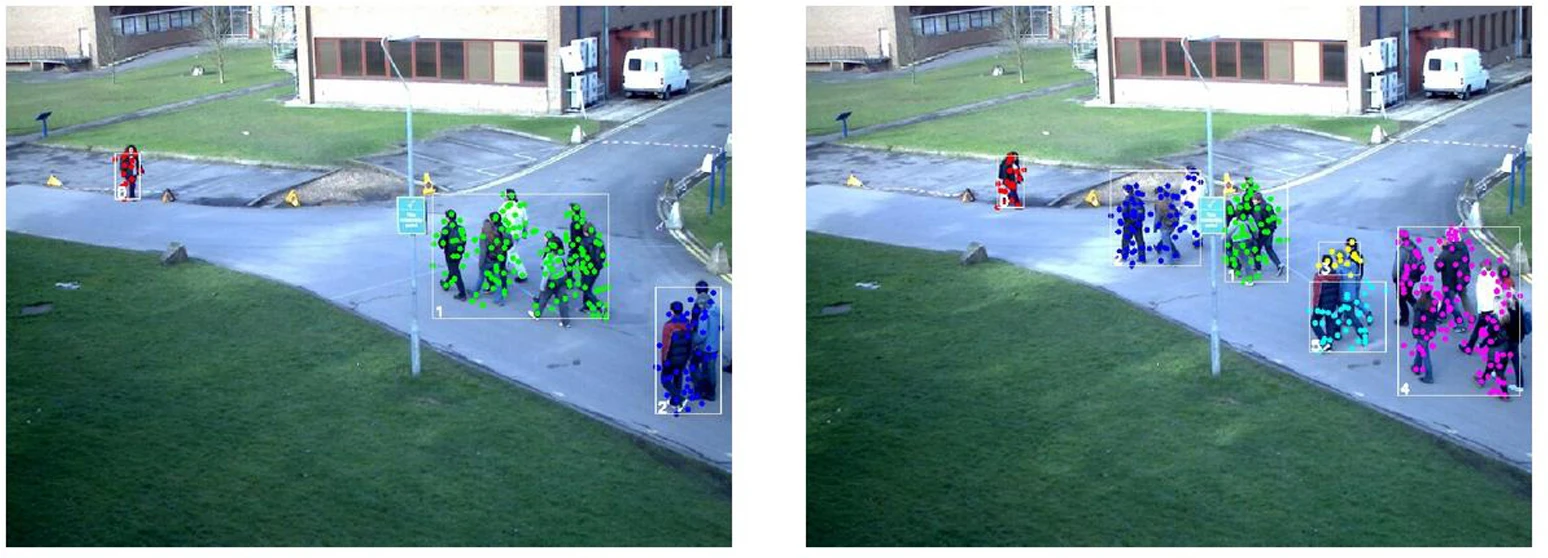
\includegraphics[width=0.8\textwidth]{Figures/history/PETS_CLUSTERS.png}
	\caption{Shlukování SURF bodů metody použité v článku 5 \cite{crowd_on_pets} (převzato z \cite{crowd_on_pets})}
	\label{fig:PETS}
\end{figure}



S narůstající popularitou neuronových sítí v oblasti strojového vidění přirozeně narůstá i množství estimátorů počítajících objekty v obraze, které jsou na neuronových sítích založeny.
S nimi se objevila i nová a dnes velmi často používaná kategorie metod pro počítání objektů v obraze, kterou je počítání lidí pomocí hustotní mapy (Density Map Estimation).

\textbf{Metody používající odhad hustotní mapy} se vyznačují tím, že konvoluční neuronová síť na základě vstupního obrazu vytvoří hustotní mapu, která popisuje odhadovanou hustotu davu v obraze, a výsledný počet lidí je stanoven na základě této mapy.

Jednoduchý příklad, jak takovou hustotní mapu vytvořit, je uveden v \cite{DeepCorn, Boominathan}.
Trénovací množina musí kromě samotných obrazů obsahovat i jejich anotace, ve kterých je pro každou hlavu, která se v daném obraze nachází, označena její pozice. Obvykle je pro tento účel použit její geometrický střed.
Anotace obrazu se dají představit jako druhý obraz \(H(x, y)\), který má ve všech bodech nulovu hodnotu, kromě bodů, které jsou geometrickým středem některé z obsažených hlav. V těchto bodech se nacházejí Diracovy impulzy \(\delta\).

%\begin{equation}
%H(x) = \sum_{i=1}^{M} \delta(x-x_i)
%\label{eq:density_map}
%\end{equation}
Pro takto anotovaný obraz je v \cite{DeepCorn, Boominathan} vytvořena základní pravda (Ground Truth) tak, že pro každý anotovaný bod je do hustotní mapy vložena normalizovaná Gaussova křivka tak, že její stření hodnota \(\mu\) je rovna pozici bodu.
V ideálním případě by byla hodnota rozptylu \(\sigma\) každé z těchto křivek odvozena od velikosti patřičné hlavy, avšak dostupné datasety tuto informaci velmi často nemají a pro každou hlavu je známa pouze její pozice.
Parametr \(\sigma\) je z toho důvodu často konstantní napříč celou hustotní mapou.
Hodnota každého bodu hustotní mapy je následně získána jako suma hodnot všech gausiánů v daném bodě, což se dá formálně zapsat jako konvoluce \(H(x, y)\) s gaussiánem.

\begin{equation}
D(x) = H(x, y) * \frac{1}{2 \pi \sigma^2} \exp{\bigg(-\frac{x^2 + y^2}{2 \sigma^2}\bigg)}
\label{eq:density_map}
\end{equation}

Pokud tuto hustotní mapu zintegrujeme určitým integrálem, tak výsledná hodnota bude rovna počtu lidí, respektive hlav, v daném obraze.
Cílem CNN je tedy naučit se co nejlépe replikovat takto vytvořené hustotní mapy pouze na základě neanotovaných vstupních obrazů.

\begin{figure}[h!]
	\centering
	\subfloat[původní obrázek]{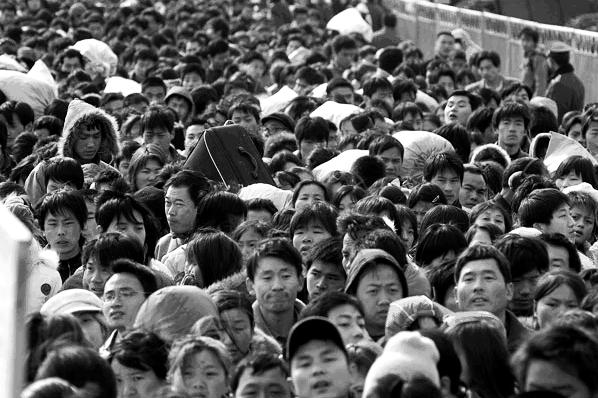
\includegraphics[width=0.4\textwidth]{Figures/history/heat_map_source.jpg}}
	\subfloat[výsledná hustotní mapa]{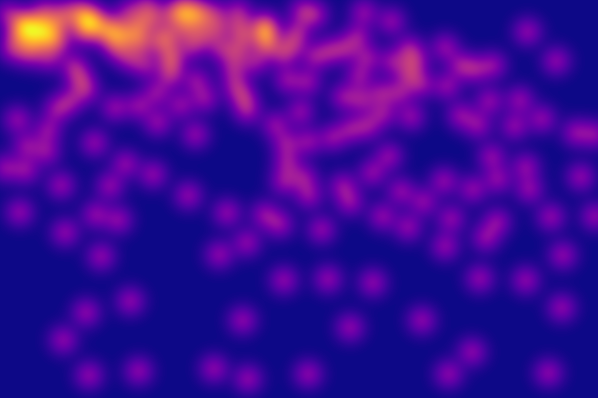
\includegraphics[width=0.4\textwidth]{Figures/history/heat_map.png}}
	\caption{Ukázka hustotní mapy vytvořené pomocí Gausiánů}
\end{figure}

Mezi sítě využívající tento přístup se řadí například M-SFANet \cite{MSFANet_for_crowd_counting}.
Obraz je dán na vstup sítě VGG-16bn \cite{VGG}, která slouží k získání příznaků.
Následně je síť rozdělena na dvě části.
Výstup z desáté vrstvy VGG je dán na vstup modulu CAN (Context-aware module) \cite{CAN_1, CAN_2}, který slouží z získání "scale-aware" příznaků a učí se jejich význam na základě jeho polohy v obraze, což pomáhá, je-li velikost lidí ve vstupním obraze výrazně ovlivněna perspektivou.
Výstup z třinácté vrstvy VGG je vložen na vstup ASPP \cite{ASPP} (Atrous spatial pyramid pooling) modulu, který podobně jako CAN slouží k extrakci "multi scale" příznaků, avšak narozdíl od CAN je jejich důležitost napříč celým obrazem stejná.
Výstupy z těchto modulů jsou vloženy do dvou dekodérů, které slouží vytvoření hustotní a pozornostní mapy (attention map).
Hustotní mapa je vytvořena stejně, jako již výše popsaná, a pozornostní mapa je vytvořena tak, že je-li hodnota v hustotní mapě hodnota větší, než práh, který je stanovený na hodnotu 0,001, tak je hodnota v pozornostní mapě rovna 1, jinak je hodnota rovna 0.
Výsledná hustotní mapa je rovna Hadamardově součinu těchto dvou map.

\begin{figure}[h!]
	\centering
	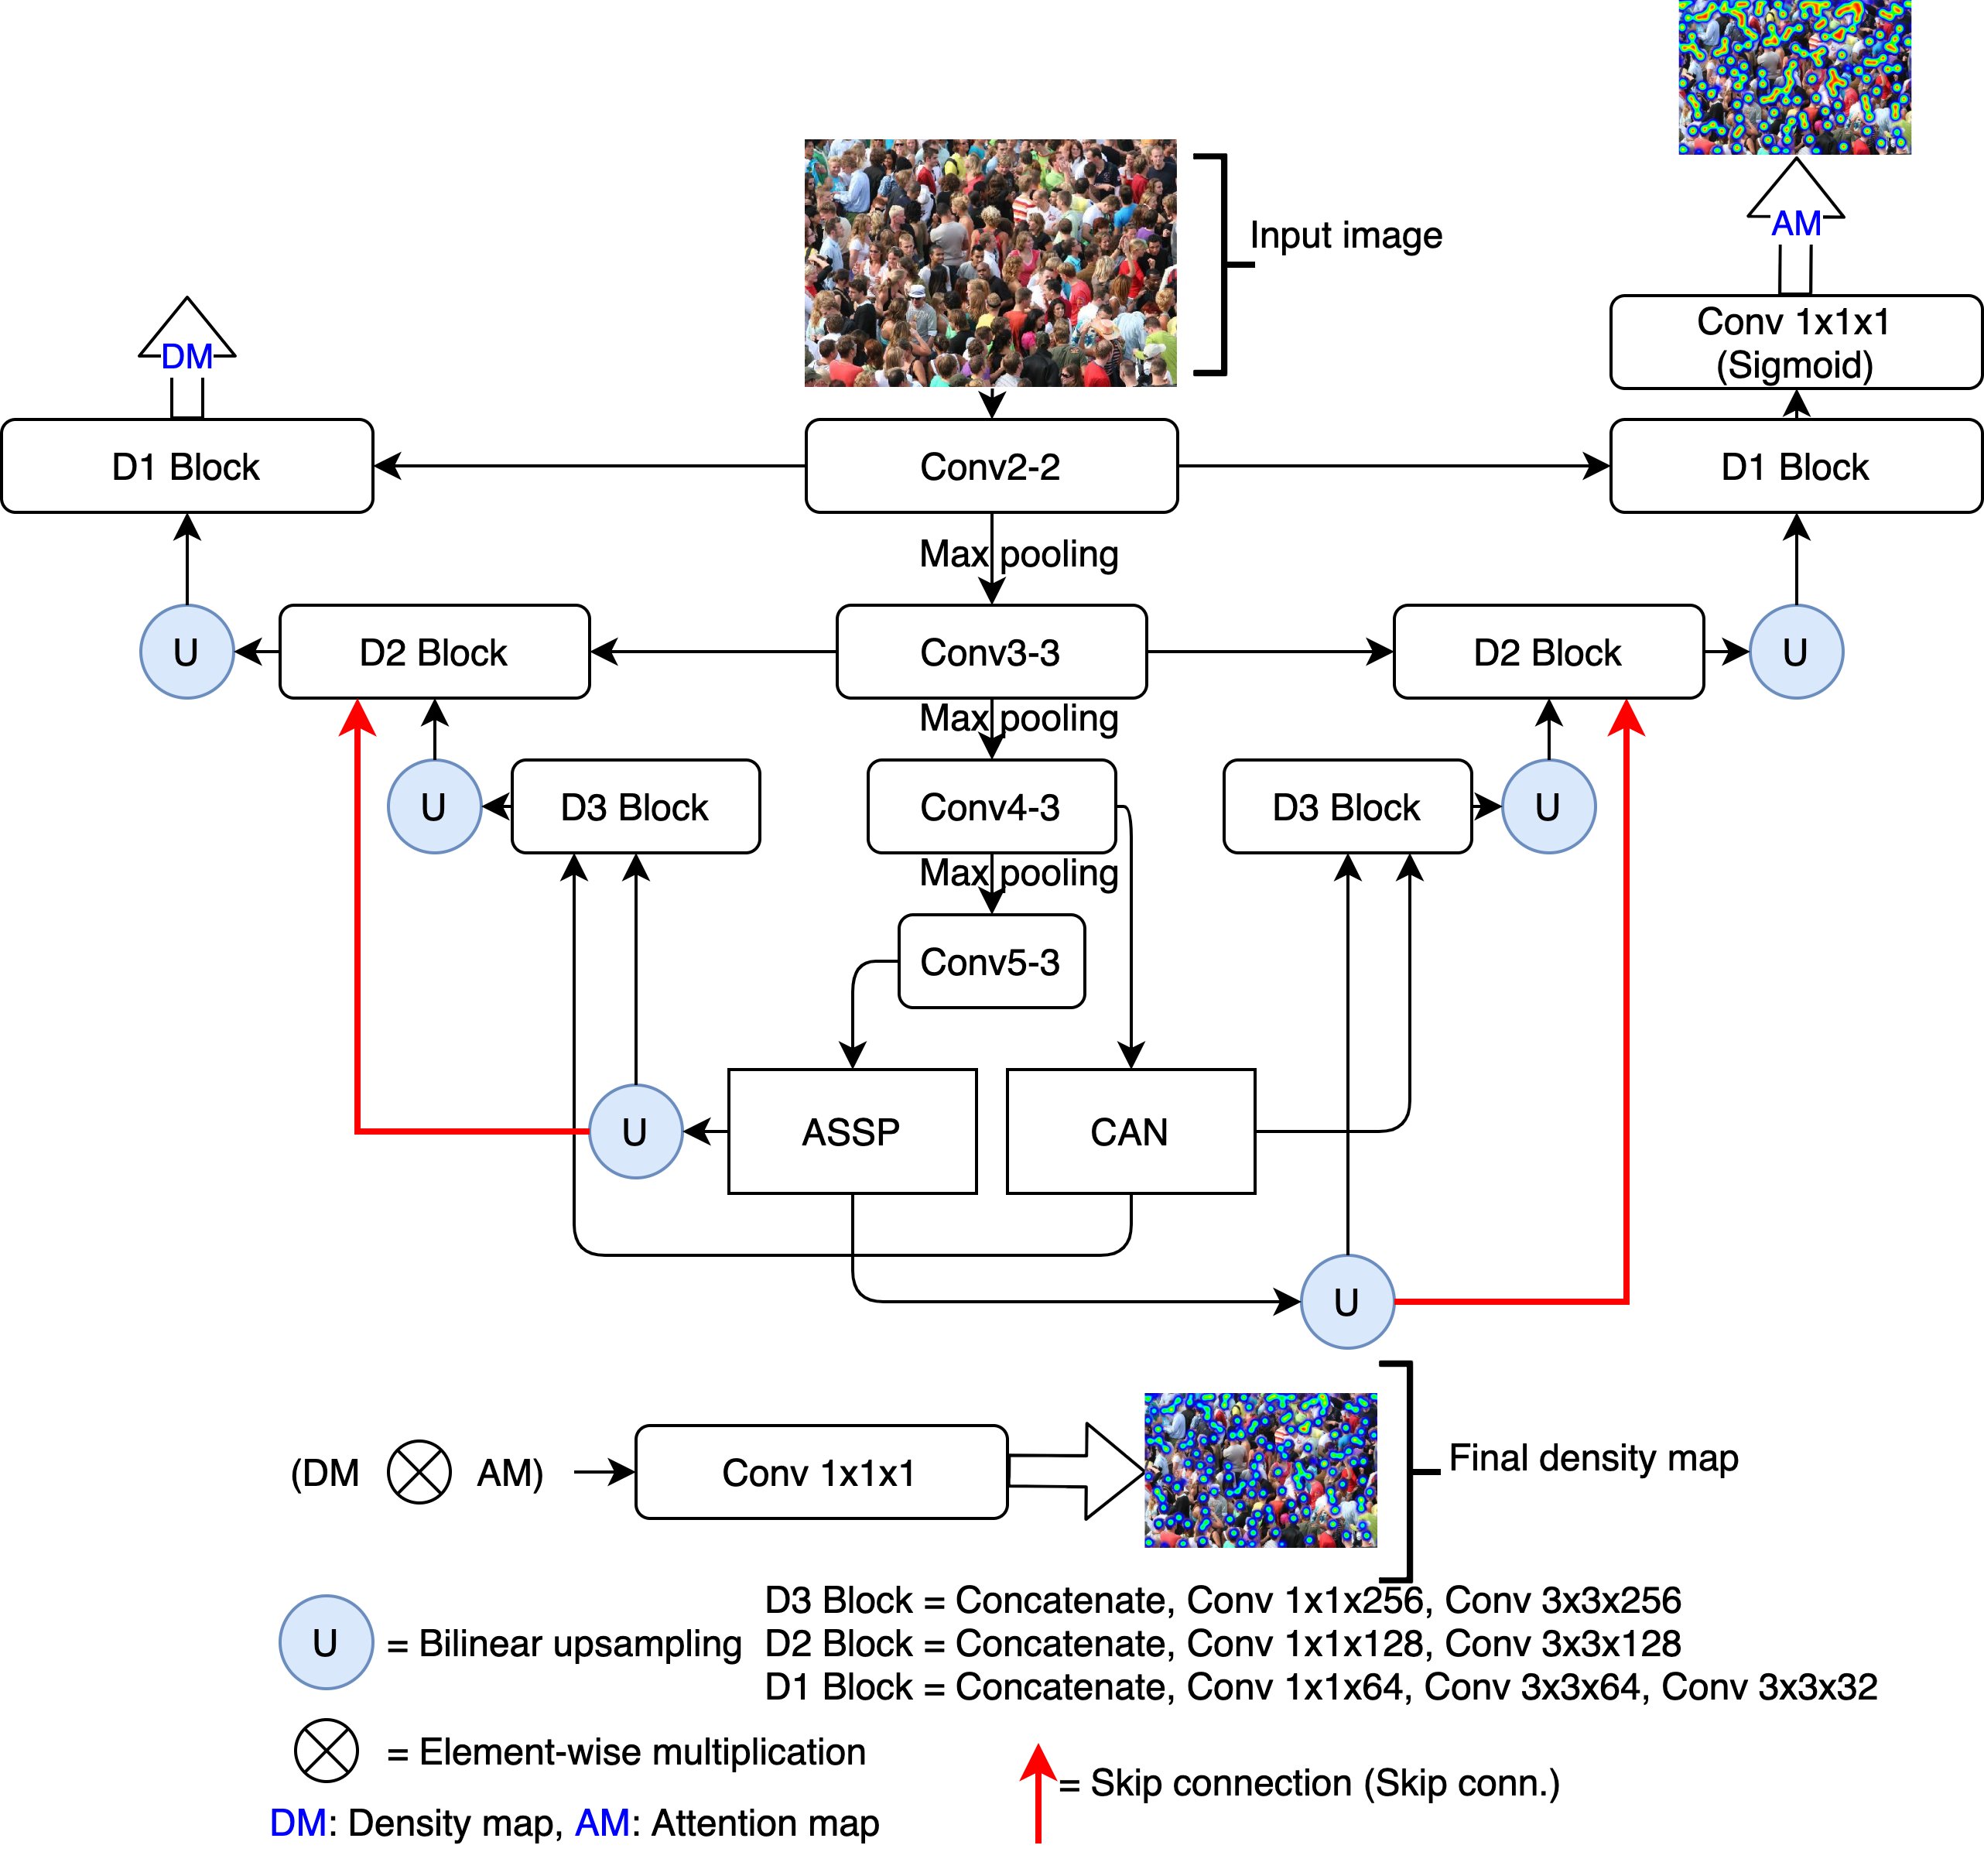
\includegraphics[width=0.6\textwidth]{Figures/history/MSFANet.png}
	\caption{Struktura sítě M-SFANet (převzato z \cite{MSFANet_for_crowd_counting})}
	\label{fig:M-SFANet}
\end{figure}







\endinput
\chapter{Navržené řešení}
\label{sec:Propesed_solution}




\endinput
\chapter{Dostupné datasety}
\label{sec:Datasets}
Před použitím konvoluční neuronové neuronové sítě navržené v této práci je nutné, aby byly váhy jednotlivých konvolucí správně nastaveny.
K tomuto účelu slouží tzv. trénovací množina.
Jedná se o množinu příkladů situací, na které může neuronová síť při svém fungování narazit.
V tomto případě, jelikož cílem sítě je určit počet lidí ve videosekvenci, se jedná o obrazy, resp. sekvenci po sobě jdoucích snímků.
Kromě samotných snímků potřebuje ještě síť základní pravdu, což je informace, pomocí které dokáže určit, jak moc se při svých predikcích mýlí, aby na základě této chyby mohla přenastavit své váhy, čímž tuto chybu sníží a posune se blíže optimu.
Tento typ strojového učení, kdy je pro natrénování modelu použita oanotovaná trénovací sada, se nazývá učení s učitelem.

Jelikož při samotném používání neuronové sítě již nedochází k žádnému přenastavování jejích vah, je pro zajištění jejího dobrého fungování naprosto stěžejní, aby byla trénovací množina rozsáhlá a co nejvíce různorodá.
Pokud je například síť natrénovaná pouze na snímcích získaných během dne, tak není zaručeno, že síť bude dosahovat stejně dobrých výsledků i na nočních záběrech.
Stejně tak model, natrénovaný na záběrech z bezpečnostních kamer, které jsou většinou umístěny vysoko nad lidskými hlavami, může mít problémy se záběry lidí pořízenými kamerou ve výšce očí.

Jelikož počítání lidí v obraze je mezi výzkumníky celkem populární problém, existuje k němu celá řada obsáhlých datasetů, z nichž některé jsou blíže popsány v této kapitole.
Mezi jednotlivými datasety ale mohou být veliké rozdíly a to nejen v rozlišení obsažených snímků, nebo velikosti davů, které snímky obsahují.
Rozdíly mohou být i v tom, jak jsou jednotlivé snímky anotovány, nebo v technologiích použítých pro pořízení těchto snímků.
To může být způsobeno například tím, kde má být daný estimátor nasazen, což bude určovat, jaké typy snímků bude dataset obsahovat.
Například datasety VisDrone \cite{VisDrone-Dataset-1, VisDrone-Dataset-2}, slouží k učení detekce, sledování a počítání objektů a lidí v obrazech a videích pořízených z dronu letícího desítky metrů nad zemí.
Oproti tomu snímky datasetu ShanghaiTechRGBD \cite{ShanghaiTechRGBD-1, ShanghaiTechRGBD-2} byly pořízeny ve zhruba dvoumetrové výšce pomocí RGB-D senzoru, což znamená, že kromě barevné složky snímky obsahují i hloubkovou informaci říkající, jak daleko od kamery se jednotlivé objekty ve scéně nacházejí.

\section{UCF-QNRF}
\begin{figure}[h!]
	\centering
	\subfloat[]{\includegraphics[height=3.5cm]{Figures/datasets/UCF-QNRF/img_0184.jpg}}
	\subfloat[]{\includegraphics[height=3.5cm]{Figures/datasets/UCF-QNRF/img_0222.jpg}}
	\subfloat[]{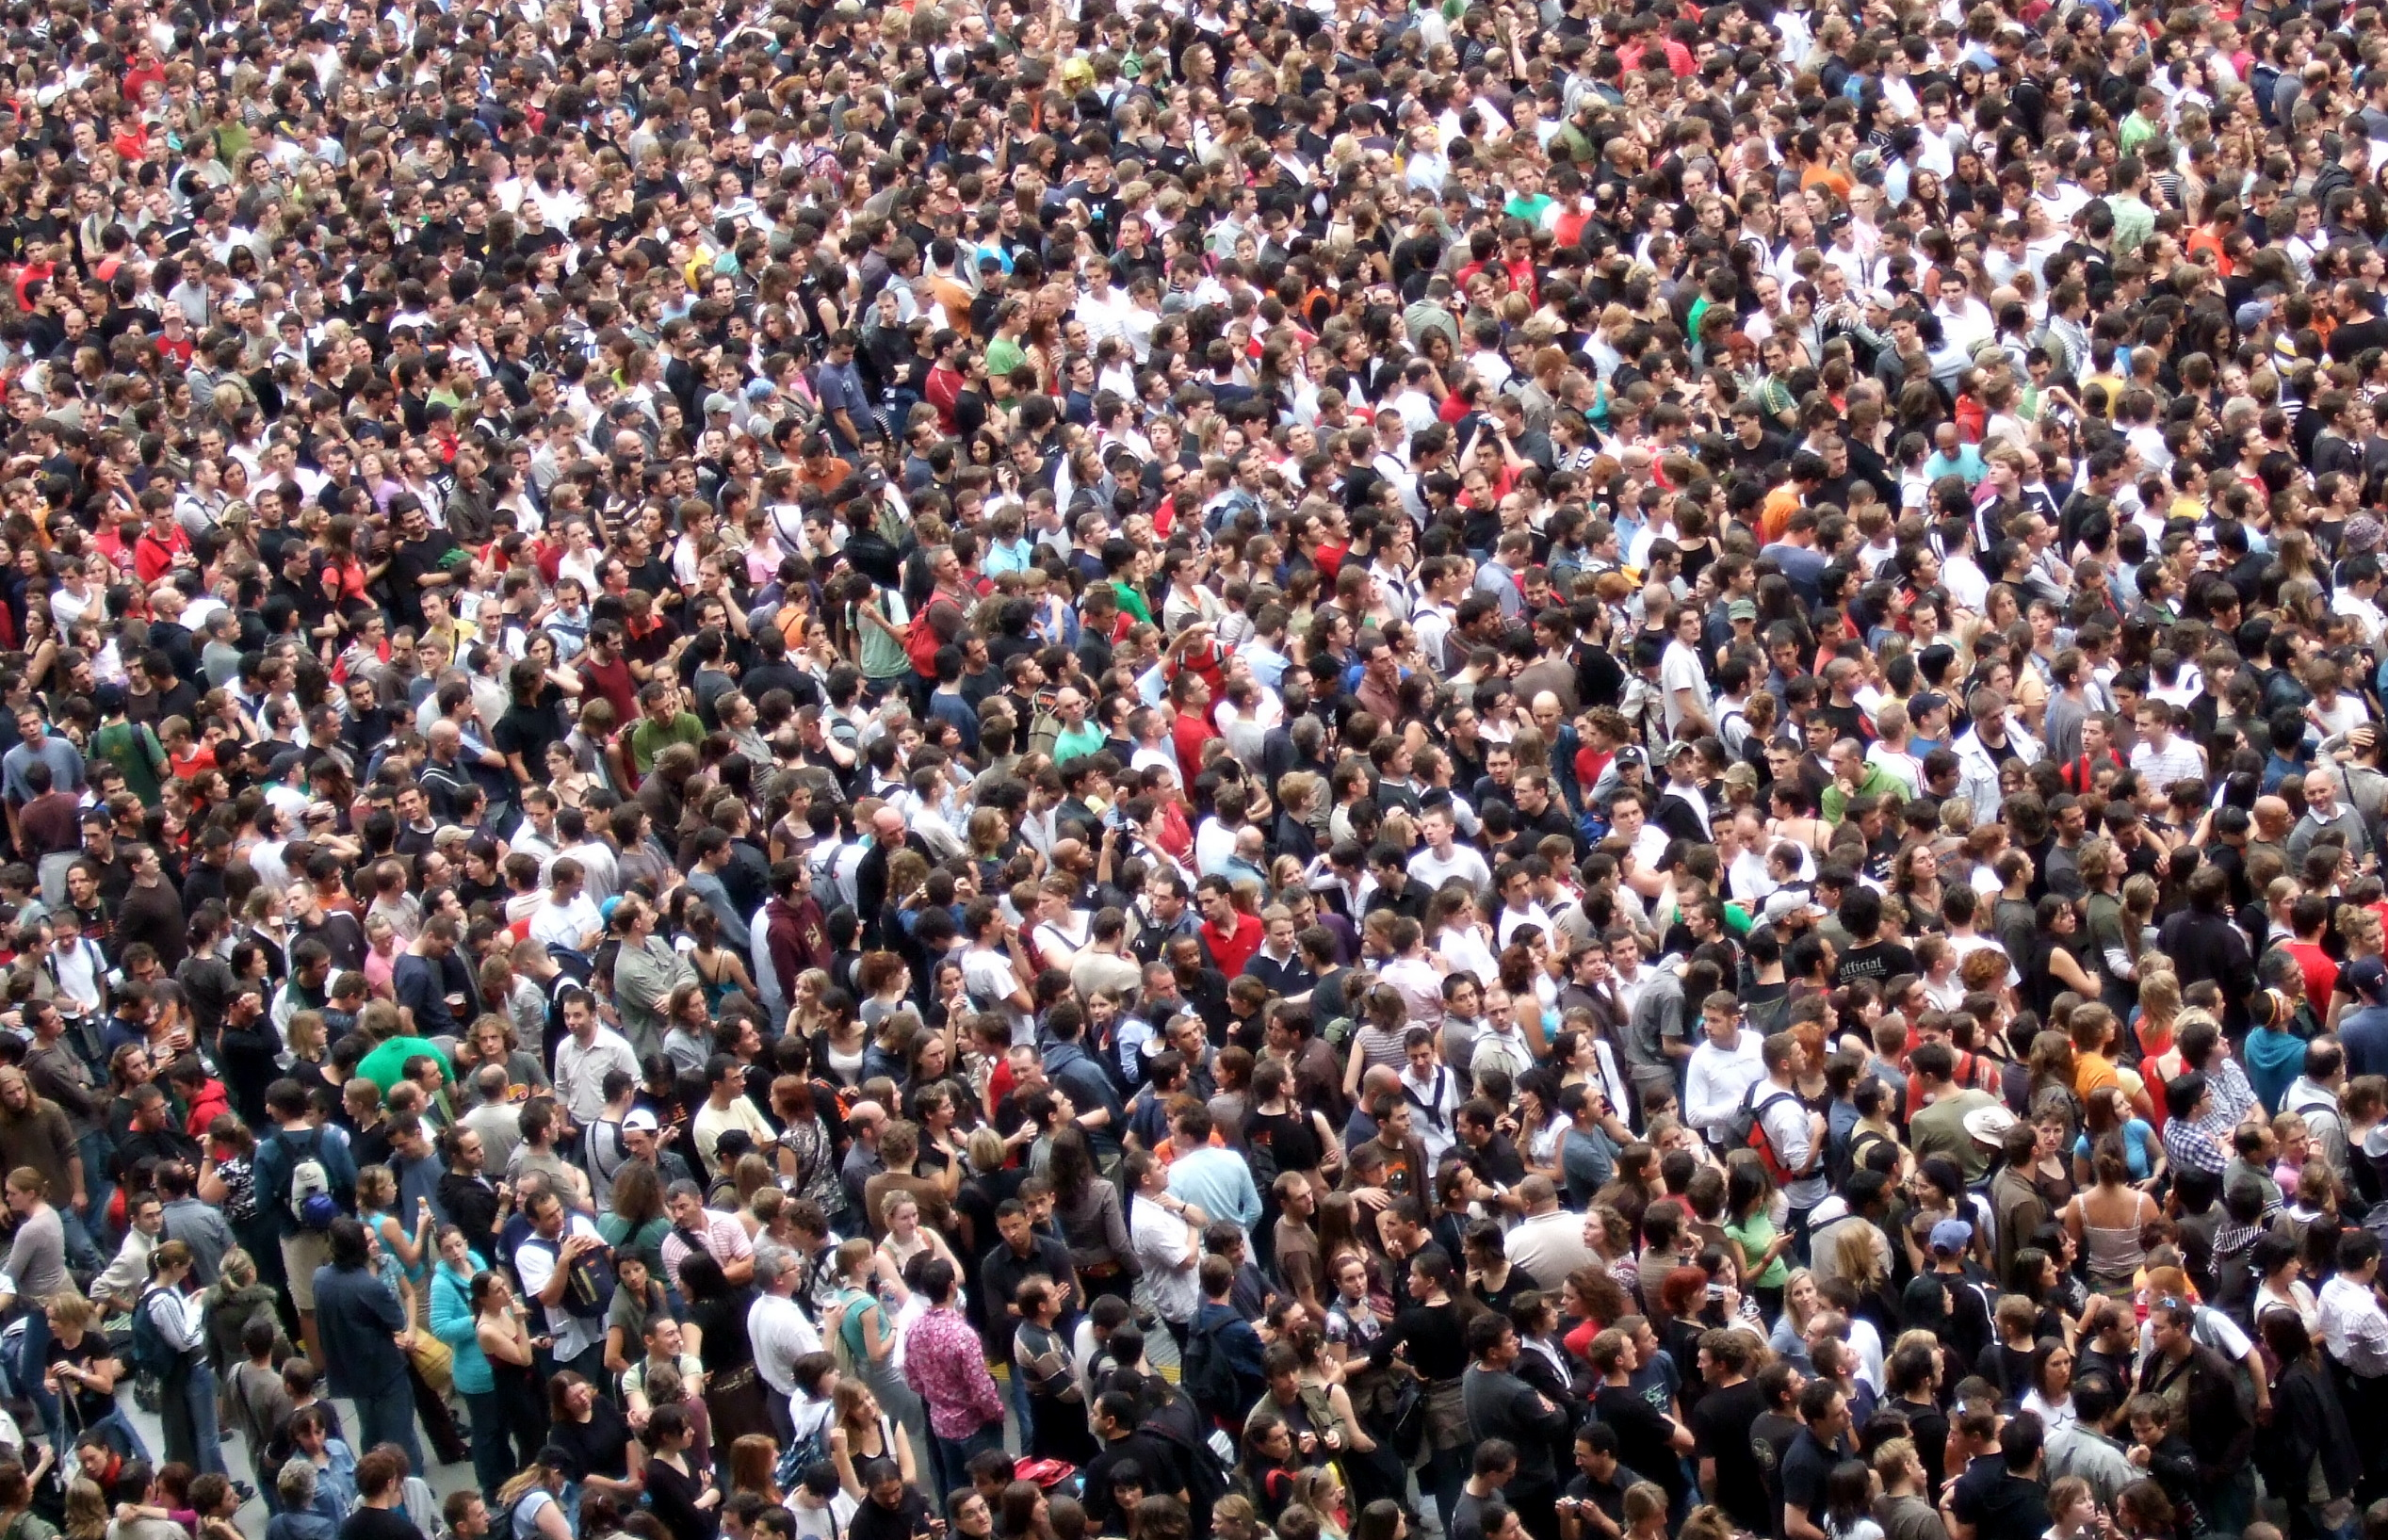
\includegraphics[height=3.5cm]{Figures/datasets/UCF-QNRF/img_0330.jpg}}
	\caption{Ukázka snímků obsažených v datasetu UCF-QNRF \cite{QNRF}}
	\label{fig:QNRF}
\end{figure}

Dataset QNRF \cite{QNRF} z Univerzity střední Floridy (University of Central Florida) je jedním z nejpopulárnějších datasetů používaných pro trénování a validaci metod strojového učení počítajících lidi v obraze.
Je totiž jedním z nejrozsáhlejších datasetů, které jsou v současnosti volně dostupné.
Celkem obsahuje 1535 na sobě nezávislých snímků získaných z internetu.
Tyto snímky jsou rozděleny na trénovací množinu obsahující 1201 snímků a testovací množinu s 334 snímky.
Populární je nejen díky své velikosti, ale také kvůli tomu, že obsahuje velkou řadu velmi hustě zalidněných scén, což ukazuje průměrný počet lidí na jednotlivých snímcích tohoto datasetu, který se rovná 815 lidí na jeden obraz.
Všechny osoby jsou ve snímcích anotovány pomocí bodů, které se nachází v pozicích odpovídajícím středům jejich hlav.
Jeho další velkou výhodou je, že fotografie v něm obsažené jsou ve vysokém rozlišení.
Průměrná velikost těchto obrazů je 5,84 megapixelů.
Augmentací dat pomocí náhodného ořezávání jde proto snadno dataset rozšířit a získat tak mnohem větší trénovací množinu, která stále obsahuje snímky v dobré obrazové kvalitě.


\section{ShanghaiTech}
Dataset ShanghaiTech \cite{ShanghaiTech} je další z v této oblasti často používaných datasetů.
Jedná se o 1198 obrázků celkem obsahujících 330 165 osob, které jsou rozděleny do dvou částí.
V části ShanghaiTech Part-A je obsaženo 482 obrázků získaných z internetu, zatímco v ShanghaiTech Part-B se nachází 716 obrázků pořízených hustě zalidněných ulicích města Shanghai. Obě části jsou dále rozděleny na testovací a trénovací množiny.
Oproti UCF-QNRF nejsou snímky tohoto datasetu uložené v tak vysokém rozlišení. Průměrné rozlišení snímků první části je 0.5 megapixelů a druhé části 0.8 megapixelů.
Průměrný počet lidí je však i zde velmi vysoký, jelikož i v tomto datasetu řada snímků zachycuje velmi husté davy lidí. V první části se na snímku nachází v průměru 501 osob a v druhé části 124 osob.
Stjeně jako v UCF-QNRF je i zde každá osoba označena pouze jediným bodem, který je umístěný v pozici středu její hlavy.

\begin{figure}[h!]
	\centering
	\subfloat[]{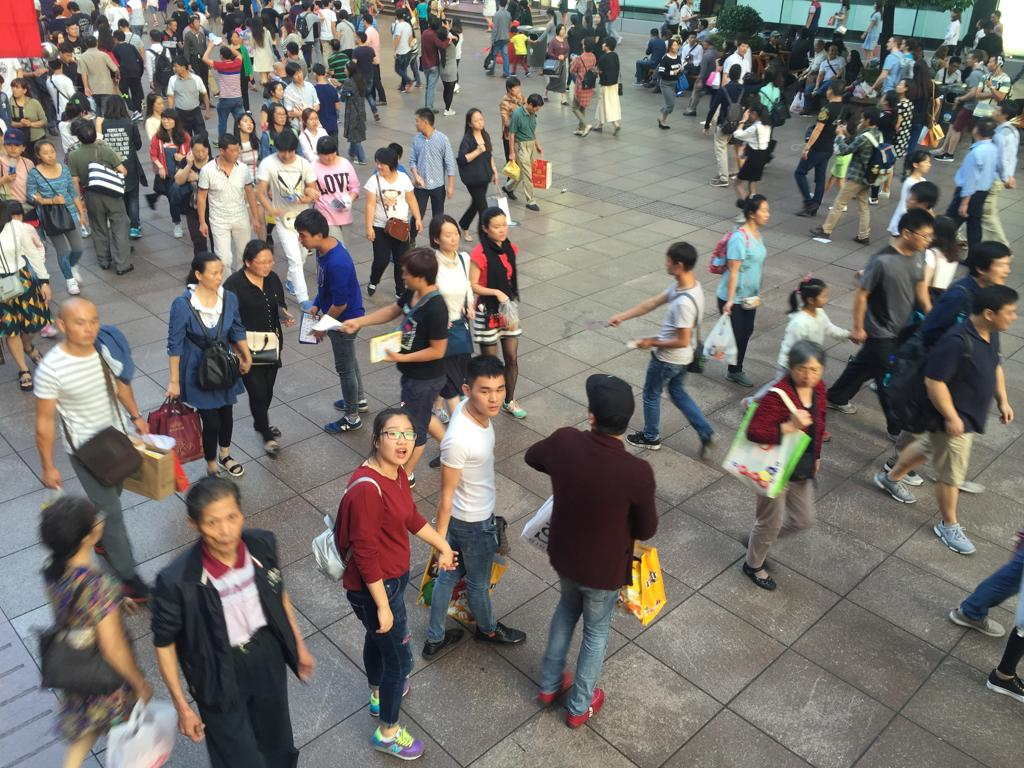
\includegraphics[height=3.5cm]{Figures/datasets/ShanghaiTech/IMG_21.jpg}}
	\subfloat[]{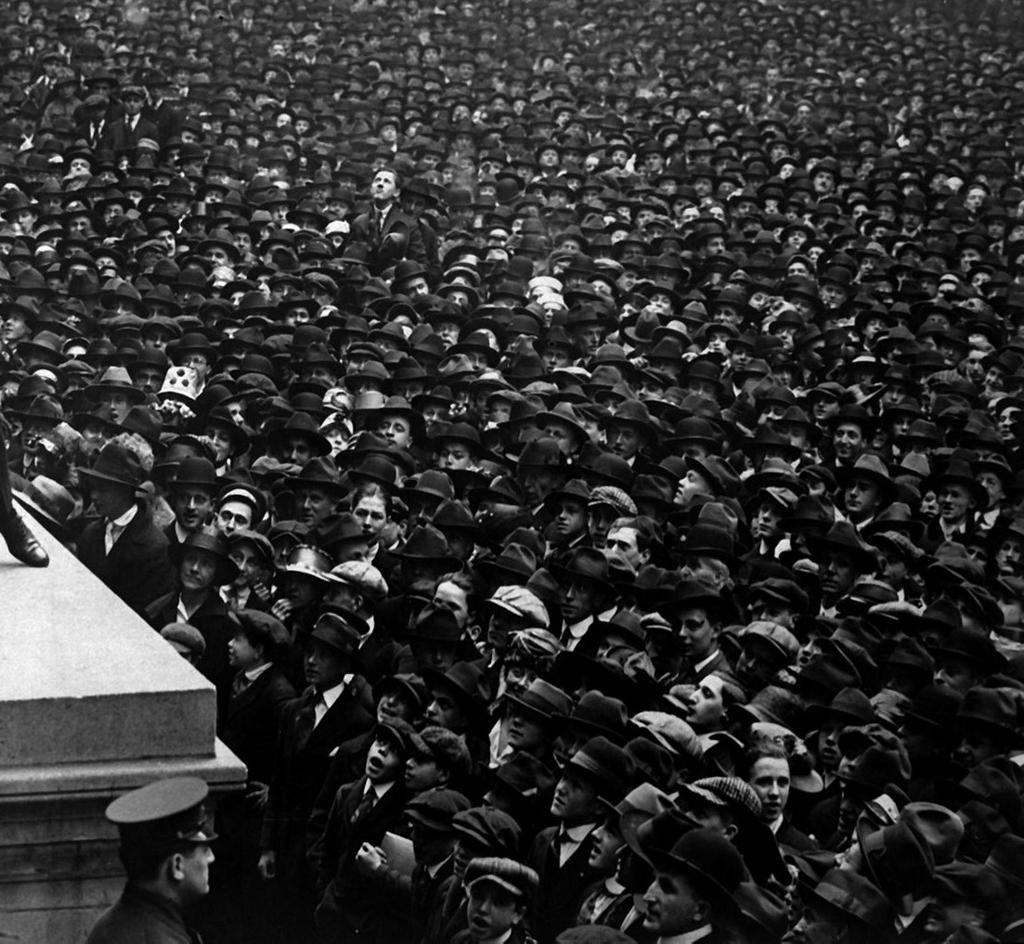
\includegraphics[height=3.5cm]{Figures/datasets/ShanghaiTech/IMG_168.jpg}}
	\subfloat[]{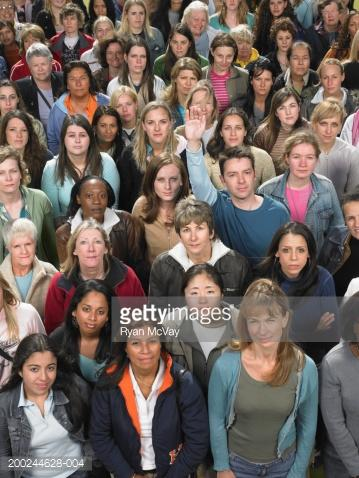
\includegraphics[height=3.5cm]{Figures/datasets/ShanghaiTech/IMG_272.jpg}}
	\subfloat[]{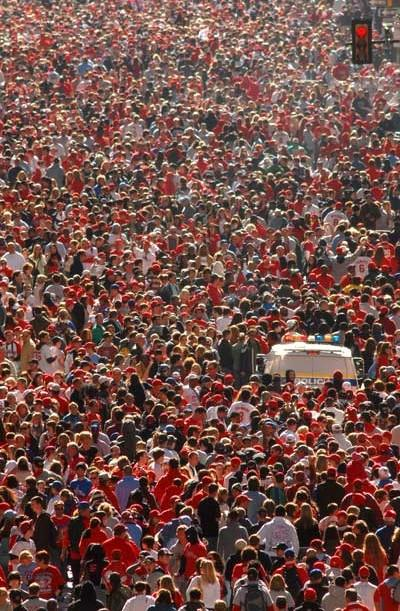
\includegraphics[height=3.5cm]{Figures/datasets/ShanghaiTech/IMG_115.jpg}}
	\caption{Ukázka snímků obsažených v datasetu ShanghaiTech \cite{ShanghaiTech}}
	\label{fig:SH_TECH}
\end{figure}


\section{Fudan-ShanghaiTech}
Převážná většina dostupných datasetů obsahuje pouze jednotlivé snímky a datasety, které obsahují videosekvence nebývají tak obsáhlé a rozmanité.

Příčinou tohoto je náročnost anotování obrazů, která nejde automatizovat a musí být proto prováděna manuálně.
Při anotování snímku musí osoba, která pro snímek vytváří základní pravdu, najít všechny lidi, kteří se v obraze nacházejí a označit jejich polohu, což je zdlouhavá činnost.
Z tohoto důvodu také datasety jako ShanghaiTech nebo UCF-QNRF používají pro označení pozic osob pouze body ve středu hlav místo obdélníků, které by vymezovaly hranice hlav, či jednotlivých osob.
Označit bod je zkrátka rychlejší, než vymezit hranice obdélníka a osoba vytvářející anotace pro obraz tak dokáže rychleji vytvořit obsáhlejší dataset.

Při anotování videí navíc přibývá problém, že pro vytvoření jediného vzorku nestačí označit lidi v jednom obraze, ale v celé sekvenci.
Pokud například estimátor počítá lidi na základě pěti po sobě jdoucích snímků, tak, aby výsledný dataset měl stejný počet položek, jako dataset obsahující pouze jednotlivé snímky, musí anotátor popsat pětkrát více snímků.

\begin{figure}[h!]
	\centering
	\subfloat[]{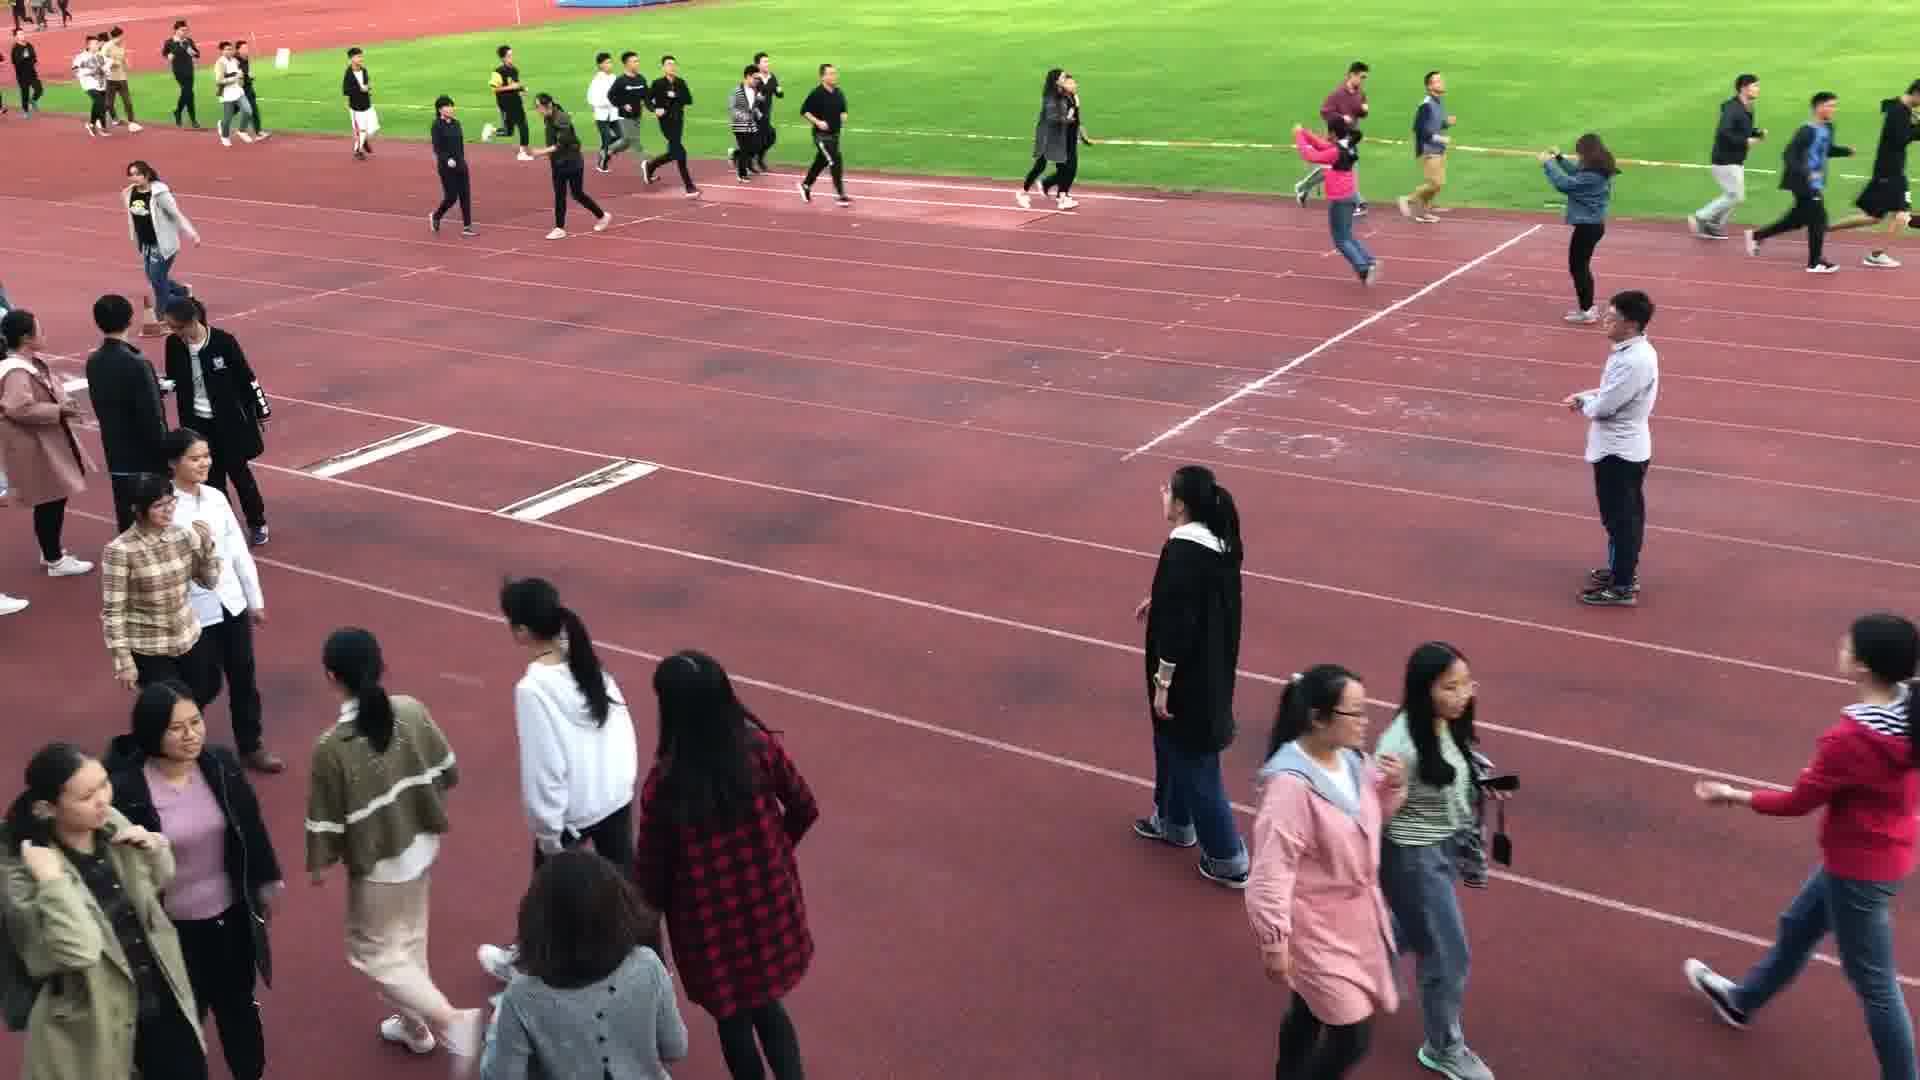
\includegraphics[width=0.45\textwidth]{Figures/datasets/FDST/015.jpg}}
	\subfloat[]{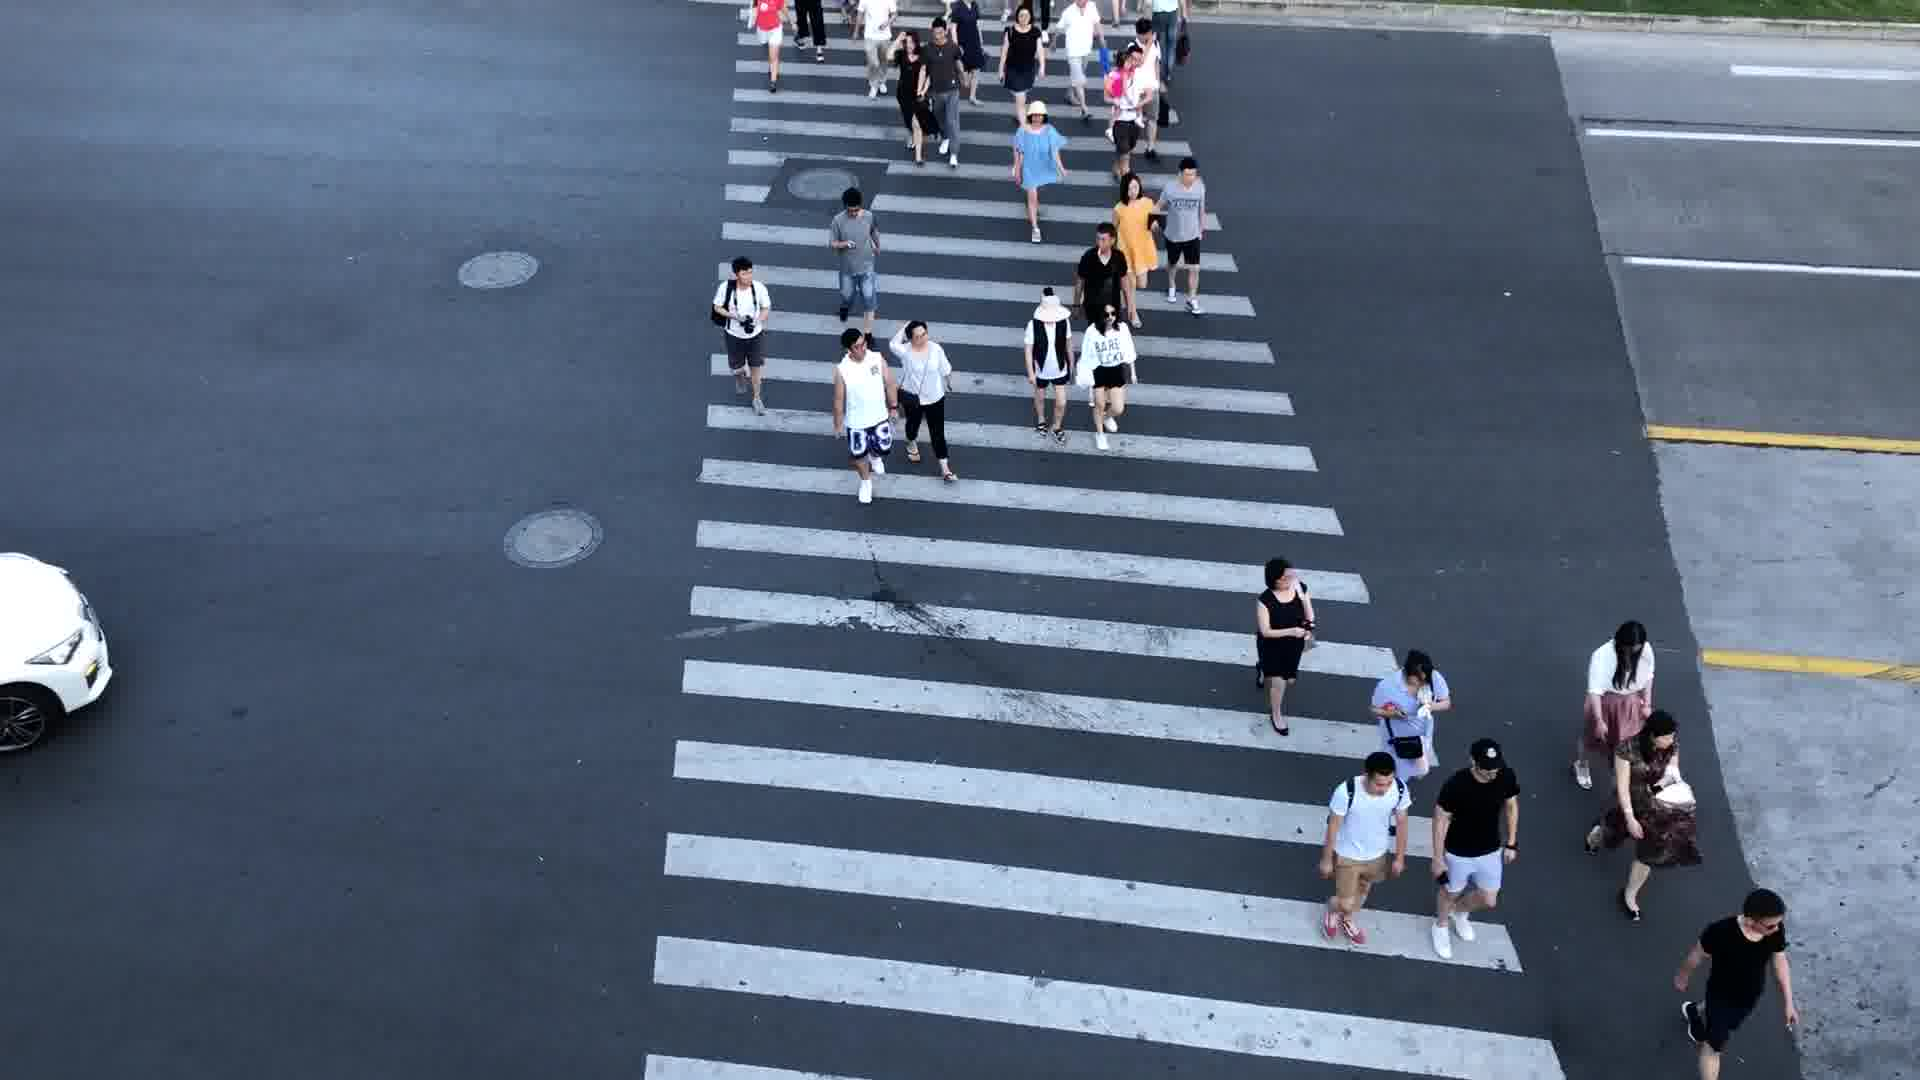
\includegraphics[width=0.45\textwidth]{Figures/datasets/FDST/150.jpg}}
	\caption{Ukázka snímků obsažených v datasetu Fudan-ShanghaiTech \cite{ShanghaiTech}}
	\label{fig:FDST}
\end{figure}


Jedním z datasetů, který se zaměřuje na videosekvence místo samostatných fotografií je Fudan-ShanghaiTech \cite{fdst_dataset}, který je tvořen videi v rozlišení 2,1 megapixelů.
Teto dataset sice celkem obsahuje 15 000 snímků, čímž do velikosti překonává UCF-QNRF, avšak je důležité zmínit, že tyto snímky jsou součástí 100 videí, které byly natočeny ve 13 různých scénách.
Rozmanitost situací, prostředí a světelných podmínek proto není tak velká, jako datasetů obsahujících fotografie.
Průměrný počet lidí na snímcích je oproti UCF-QNRF a ShanghaiTech o řád nižší. Místo stovek se zde v průměru nachází 23 lidí na jeden snímek.
Nejsou zde proto zachyceny tak husté davy a lidé jsou mnohem více separováni.
Snímky jsou anotovány pomocí obdélníků, které udávají pozice a rozměry jednotlivých hlav.

\section{GTA5 Crowd Counting Dataset}
Jak již bylo v této kapitole popsáno, sbírání a anotování rozsáhlých rozmanitých datasetů pořízených v reálném světě je časově velmi náročná činnost.
Nabízí se však ale i jiná možnost, jak vytvořit velmi rozsáhlou datovou množinu ve které známe přesnou polohu každé osoby aniž by ji musel anotátor v obraze manuálně najít.
Touto možností je použití syntetických datasetů.
Takovéto datasety neobsahují data z reálného světa, ale fabrikovaná data, která se co možná nejblíže podobají reálným.

V současnosti je počítačová grafika dostatečně pokročilá na to, aby dokázala vykreslit fotorealistickou reprezentaci scény, čehož může být využito právě pro tvorbu daného datasetu.
Jelikož taková scéna je vykreslována počítačem, známe nejen souřadnice každého člověka ve scéně, ale přesně víme, jeho postoj či jak moc je v obraze vidět a které části nejsou zakryty, díky čemuž je možné vytvořit velmi přesnou základní pravdu, a to bez použití anotátora.

To ale neznamená, že pro vytvoření takového datasetu není potřeba velké množství lidská práce.
Generátor datasetu totiž musí být schopen simulovat podmínky, ve kterých má trénovaný estimátor pracovat.
Proto, pokud je například cílem, aby estimátor pracoval ve venkovních podmínkách celý rok v každou denní hodinu, musí být schopen generátor datasetu obsahovat simulaci počasí a denního cyklu, což do něj musí někdo naimplementovat.
V datasetu by také měly být obsaženy různé aktivity, které lidé normálně dělají.
Bude-li totiž obsahovat pouze stroze stojící lidi, nejspíše bude mít problémy ve chvíli, kdy narazí na situaci, kdy se ve scéně někdo posadí, nebo začne běhat.
Generátor proto musí obsahovat celou řadu animací, které musí vytvořit a přidat do scény, nebo vytvořit nějaký systém behaviorální simulace.
Dále je podstatné i prostředí scény, do které jsou lidé vloženi.
Při použití identické scény napříč celým datasetem, může docházet k overfittingu, ke kterému by mohlo dojít i v případě, že v použitých modelech lidí není dostatek variace.
Neuronová síť by si příliš navykla na vzory v datech, které se neustále opakují, což by ve výsledku vedlo ke zhoršení výkonu estimátoru při reálném nasazení.
Jak je z tohoto patrné, vytvoření generátoru syntetického datasetu vyžaduje mnoho člověkohodin práce vysoce kvalifikovaných pracovníků, jako jsou programátoroři a výtvarníci.
Vytvoření takového generátoru datasetu je proto mnohem náročnější jak na lidský, tak i na finanční kapitál.

Existuje však mnoho softwarových děl, které řadu z těchto požadavků splňují.
V mnoha počítačových hrách se hráči pohybují v prostředích modelovaných podle reálného světa obklopeni mnoha rozličnými nehratelnými postavami.
Například ve hrách série Hitman \cite{hitman} od vývojáře IO Interactive prochází hráč mnoha úrovněmi, které jsou plné simulovaných davů čítajících stovek postav.
Aby měl hráč pocit, že simulovaný svět, ve kterém se nachází je reálný, mají tyto postavy řadu činností, které provádějí a které jsou animovány.

\begin{figure}[h!]
	\centering
	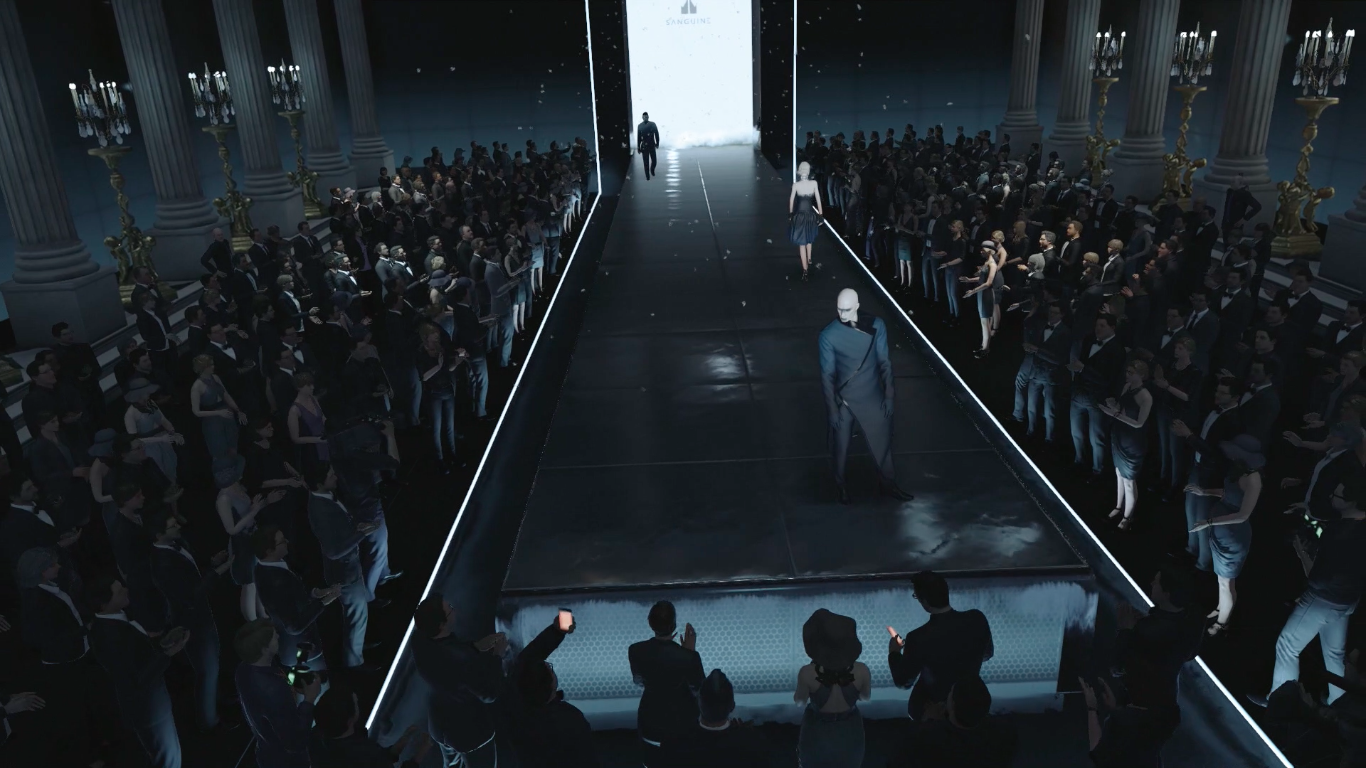
\includegraphics[width=0.7\textwidth]{Figures/datasets/GCC/Hitman_crowd.png}
	\caption{Ukázka davu ve hře Hitman (2016) (převzato z \cite{ign_2017})}
	\label{fig:RNN_architecture}
\end{figure}


Moderní počítačové hry jsou proto slibným zdrojem dat pro trénování neuronových sítí.
Totu problematikou se zabývá i článek Learning from Synthetic Data for Crowd Counting in the Wild \cite{GCC_dataset}. 
Pro účely této práce vytvořili autoři dataset GTA5 Crowd Counting Dataset (GCC), který využívá hry Grand Theft Auto V \cite{GTAV} pro vytvoření syntetických scén.
Tato hra nabízí 252 čtverečních kilometrů terénu, simulaci počasí i denního a nočního cyklu a postavy mohou být oděny do mnoha různých druhů oblečení, mohou mít řadu účesů.
Dataset proto může být velmi rozmanitý.

Celkem dataset GCC sestává z 15 212 snímků pořízených ve 400 různých scénách za různých meteorologických a světelných podmínek a celkem obsahujících 7 625 843 osob.
Každá osoba je ve snímku anotována pomocí bodu umístěného do středu její hlavy.

\begin{figure}[h!]
	\centering
	\subfloat[]{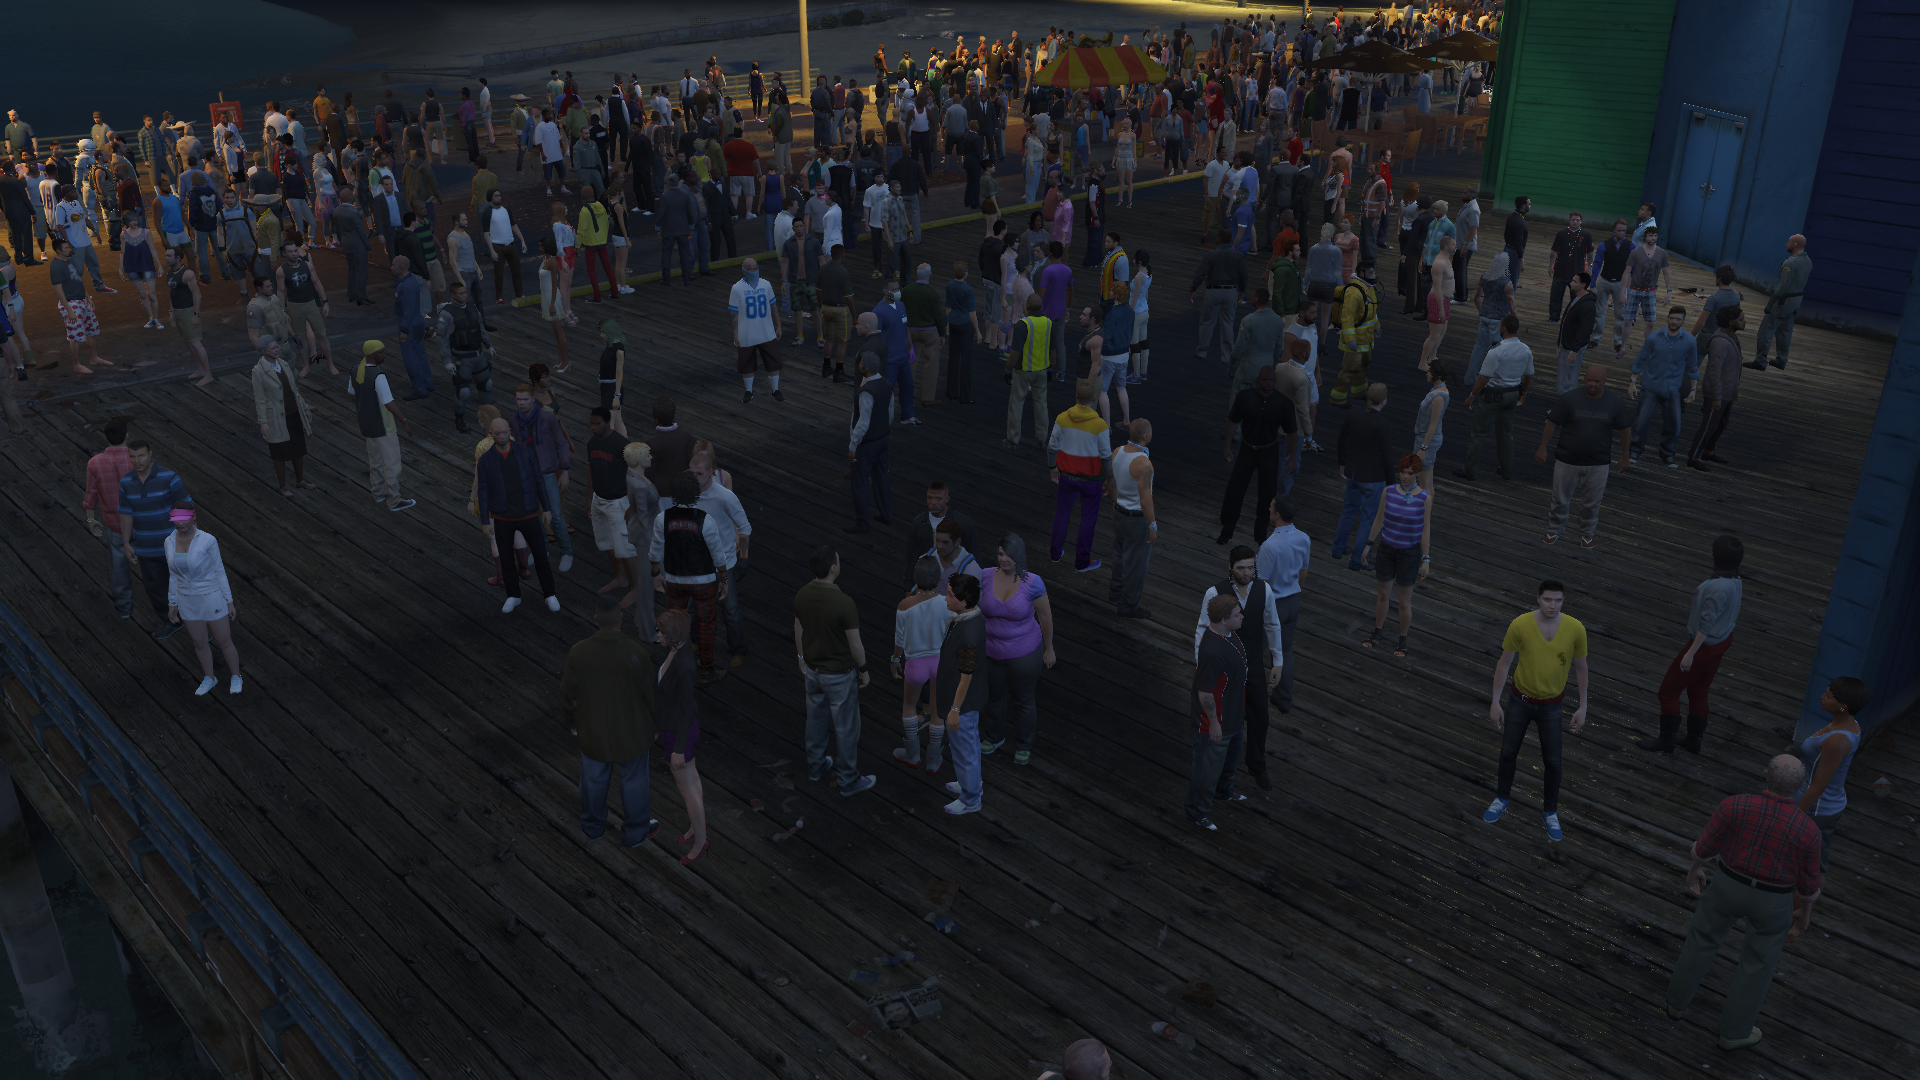
\includegraphics[height=4cm]{Figures/datasets/GCC/GCC_1.png}}
	\subfloat[]{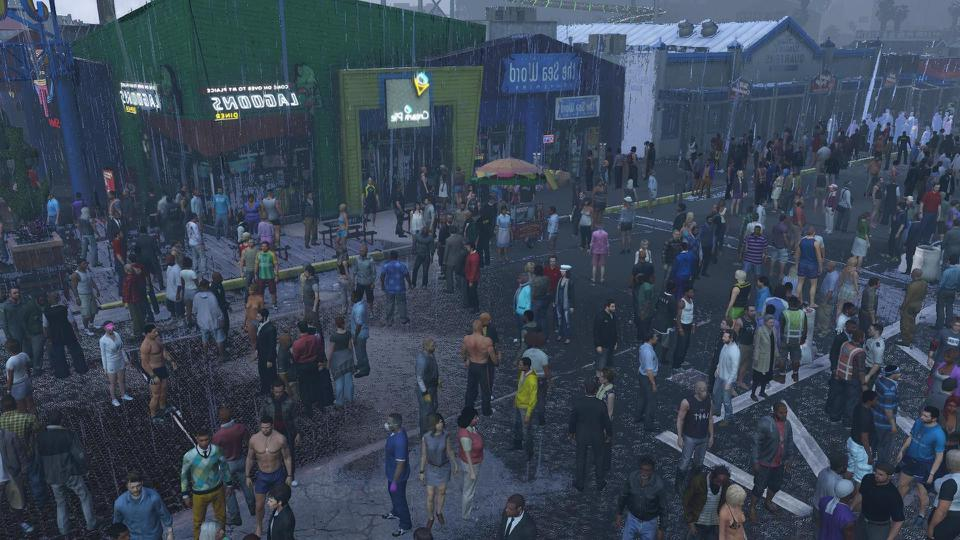
\includegraphics[height=4cm]{Figures/datasets/GCC/GCC_2.jpg}}
	\caption{Ukázka snímků obsažených v datasetu GCC \cite{GCC_dataset}}
	\label{fig:QNRF}
\end{figure}

Při pohledu na snímky tohoto datasetu je ale očividné, že se jedná o uměle vykreslenou scénu.
Autoři článku proto navrhují postup, jak vygenerovaný dataset upravit, aby se blíže podobal reálným datům.
Tohoto dosahují pomocí neuronové sítě typu GAN (Generative adversarial network), jejímž cílem je syntetické obrazy upravit tak, aby se vzhledem více podobaly obrazům obsaženým v datasetech z reálného světa.
Samotný estimátor je potom trénován až s pomocí takto upravených fotografií.






\begin{table}[h!]
\centering
\begin{tabular}{|l|r|r|l|}
\hline
                    & \begin{tabular}[c]{@{}l@{}}počet\\ snímků\end{tabular} & \begin{tabular}[c]{@{}l@{}}průměrný počet\\ lidí na snímku\end{tabular} & \begin{tabular}[c]{@{}l@{}}průměrné\\ rozlišení snímku {[}px{]}\end{tabular} \\ \hline
UCF-QNRF            & 1 535                                                   & 815                                                                     & 2013 * 2902                                                                  \\ \hline
ShanghaiTech Part-A & 482                                                    & 501                                                                     & 589 * 868                                                                    \\ \hline
ShanghaiTech Part-B & 716                                                    & 124                                                                     & 768 * 1024                                                                   \\ \hline
Fudan-ShanghaiTech  & 15 000                                                 & 26                                                                      & 1080 * 1920                                                                  \\ \hline
\end{tabular}
\end{table}

\endinput
\chapter{Implementace navrženého řešení}
Pro implementaci modelu navrženého v této práci, byl použit jazyk Python 3, který byl zvolen z důvodu jeho popularity v oblastech strojového učení a zpracování obrazu, což je dáno a zároveň také způsobuje dostupnost celé řady rozsáhlých a pokročilých knihoven, které práci v těchto oblastech výrazně ulehčují.
Sice se jedná o vysokoúrovňový interpretovaný jazyk, což vede k nižšímu výkonu oproti aplikacím, které jsou psány v jazycích jako Rust nebo C, avšak tento nedostatek je často kompenzován samotnými knihovnami, které jsou implementovány právě v těchto nízkoúrovňových jazycích.
Python 3 navíc nabízí velmi expresivní syntaxi, která umožňuje velmi rychlý a pohodlný vývoj, což jej činí ideálním jazykem pro rychlé softwarové prototypování.
Z těchto důvodů se stal velmi populárním v akademické sféře, kde k prototypování aplikací využívajících strojové učení dochází velmi často.
Toto se projevuje i v řadě článků, ze kterých bylo v této práci čerpáno, kde ukázkové zdrojové kódy byly často implementovány právě v Pythonu.

Jak již bylo řečeno, tento jazyk nabízí široký ekosystém knihoven a frameworků pro strojové učení a práci s neuronovými sítěmi.
Do této kategorie spadá například TensorFlow \cite{tensorflow}, Keras \cite{Keras} nebo PyTorch \cite{PyTorch}.
Právě poslední zmíněný framework byl vybrán pro implementaci neuronové sítě navržené v kapitole \ref{sec:Propesed_solution}.
Jedná se o open source framework, jehož cílem je zjednodušit vytváření a učení komplexních hlubokých neuronových sítí a jedná se o jeden z nepoužívanějších nástrojů v této oblasti.
To dokazuje i jeho nasazení ve velkých technologických společnostech, jako jsou Tesla, META, NVIDIA nebo Amazon.
Primárně je určen pro použití s jazykem Python, avšak nabízí i rozhraní pro C++ a jiné jazyky, takže v případě, že programátor chce výslednou aplikaci co nejvíce výkonnostně vyladit, či použít implementovaný model v aplikaci založené na jiných technologiích, může využít právě tohoto rozhraní.
Jeho velikou výhodou je snadné použití GPU akcelerace pro složité operace s tenzory, což je základní datová struktura, se kterou PyTorch pracuje.
Programátor tak pomocí tohoto frameworku může velmi snadno a rychle vytvořit komplexní neuronovou síť a snadno ji natrénovat.

\begin{figure}[h!]
	\centering
	\subfloat[logo programovacího jazyka Python]{
\includegraphics[height=3.5cm]{Figures/implementation/python_logo.pdf}}
	\hspace{0.2\textwidth}
	\subfloat[logo frameworku PyTorch]{
\includegraphics[height=3.5cm]{Figures/implementation/pytorch_logo.pdf}}
	\caption{loga použitých technologií}
	\label{fig:logos}
\end{figure}

\section{Načítání vstupu a augmentace dat}
Jelikož část sítě používá rekurentní LSTM buňky, je nutné, aby vstupem takové sítě byla sekvence po sobě jdoucích obrazů.
Výstup buňky totiž nezáleží pouze na aktuálním vstupu, ale i na kontextu získaném ze vstupů předchozích.
Stejně tak i při adaptaci neuronů během trénování sítě, se musí nastavit i váhy mezi neuronem a skrytými stavy.
Jelikož je výstpu neuronu závislý i na stavech předchozích, tak změna jeho vah je závislá nejen na chybě aktuální, ale i chybách v následujících krocích sekvence.
Proto i při trénování sítě je nutné, aby vstupy, pomocí kterých je síť trénována, byly ve formě sekvence.





\endinput
\chapter{Testování a výsledky}
\label{sec:Testing}

Navržená neuronová síť byla testována na sestavě s Linuxovou distribucí Ubuntu 21.10 a obsahující osmijádrový procesor AMD Ryzen 7 5800H, 16 GB RAM a grafickou kartu NVIDIA GeForce RTX 3060 6GB GDDR6.
Právě velikost grafické paměti se při testování sítě ukázala jako největší limitace.
Při akceleraci operací neuronové sítě pomocí grafické karty jsou model i právě zpracovávané data nahrány v grafické paměti, kde za běhu aplikace zabírají kolem pěti GB paměti. 
Na grafické kartě tak zůstávaly řádově stovky MB volné paměti, která bývá navíc z části zabraná systémovými aplikacemi, což nedávalo mnoho místa pro větší zesložitění architektury sítě.

Hlavním cílem testování bylo zjistit, jaký vliv má použití sekvence více snímků na vstupu na přesnost výsledného počtu.
Z toho důvodu bylo natrénováno několik modelů, které se lišily hodnotou parametru \texttt{sequence\_length} udávajícího délku vstupní sekvence, ze které model estimuje počet lidí v jejím posledním obraze.
Stejnou délku měly i sekvence v trénovací množině pomocí kterých byl estimátor natrénován.

Aby se lidskému mozku videosekvence zdály plynulé, jsou při snímání kamerou snímkovány s poměrně vysokou frekvencí. 
Ta může u klasického videa dosahovat například dosahovat hodnoty třicet snímků za sekundu, což znamená, že časový rozdíl mezi jednotlivými snímky je zhruba 0,03 sekundy.
Lidé jsou navíc poměrně pomalu se pohybující stvoření.
Člověk, který jde rychlostí \(4 kmh^{-1}\) se tak za třicetinu sekundy pohne o \(3,5 cm\).
Efekt tohoto pohybu v obraze také bude velmi záviset na tom, jak daleko od kamery se daná osoba nachází. 
V případě, že by scéna byla snímána kamerou s horizontálním rozlišením 1080 pixelů a s objektivem s ekvivalentní ohniskovou vzdáleností \(50 mm\), by člověk jdoucí kolmo ke směru pohledu kamery a vzdálený od ní 10 metrů urazil za třicetinu sekundy vzdálenost ekvivalentní 2,3 pixelů.
Je proto zřejmé, že rozdíly mezi dvěma po sobě jdoucími snímky proto budou minimální a bude v sekvenci tak bude obsaženo velké množství redundantních informací.
Z tohoto důvou byl u trénovaných sítí měněn i parametr \texttt{stride}, který udává krok mezi snímky v sekvenci.
Je-li hodnota tohoto parametru rovna jedné, nebudou mezi snímky v sekvenci žádné mezery a budou brány tak, jak se ve vstupním videu nacházejí.
V případě, že má tento parametr hodnotu dva, tak již bude jeden snímek přeskočen a v sekvenci se tak bude nacházet každý druhý snímek ze vstupního videa.






\endinput

% Seznam literatury
\printbibliography[title={Literatura}, heading=bibintoc]


\end{document}
